% A LaTeX template for EXECUTIVE SUMMARY of the MSc Thesis submissions to 
% Politecnico di Milano (PoliMi) - School of Industrial and Information Engineering
%
% https://www.ingindinf.polimi.it/it/didattica/lezioni-e-esami/esami-di-laurea-e-laurea-magistrale
%
% S. Bonetti, A. Gruttadauria, G. Mescolini, A. Zingaro
% e-mail: template-tesi-ingind@polimi.it
%
% Last Revision: October 2021
%
% Copyright 2021 Politecnico di Milano, Italy. NC-BY

\documentclass[11pt,a4paper,twocolumn]{article}

%------------------------------------------------------------------------------
%	REQUIRED PACKAGES AND  CONFIGURATIONS
%------------------------------------------------------------------------------
% PACKAGES FOR TITLES
\usepackage{titlesec}
\usepackage{color}

% PACKAGES FOR LANGUAGE AND FONT
\usepackage[utf8]{inputenc}
\usepackage[english]{babel}
\usepackage[T1]{fontenc} % Font encoding

% PACKAGES FOR IMAGES
\usepackage{graphicx}
\graphicspath{{Images/}} % Path for images' folder
\usepackage{eso-pic} % For the background picture on the title page
\usepackage{subfig} % Numbered and caption subfigures using \subfloat
\usepackage{caption} % Coloured captions
\usepackage{transparent}

% STANDARD MATH PACKAGES
\usepackage{amsmath}
\usepackage{amsthm}
\usepackage{bm}
\usepackage[overload]{empheq}  % For braced-style systems of equations

% PACKAGES FOR TABLES
\usepackage{tabularx}
\usepackage{longtable} % tables that can span several pages
\usepackage{colortbl}

% PACKAGES FOR ALGORITHMS (PSEUDO-CODE)
\usepackage{algorithm}
\usepackage{algorithmic}

% PACKAGES FOR REFERENCES & BIBLIOGRAPHY
\usepackage[colorlinks=true,linkcolor=black,anchorcolor=black,citecolor=black,filecolor=black,menucolor=black,runcolor=black,urlcolor=black]{hyperref} % Adds clickable links at references
\usepackage{cleveref}
\usepackage[square, numbers, sort&compress]{natbib} % Square brackets, citing references with numbers, citations sorted by appearance in the text and compressed
\bibliographystyle{plain} % You may use a different style adapted to your field

% PACKAGES FOR THE APPENDIX
\usepackage{appendix}

% PACKAGES FOR ITEMIZE & ENUMERATES 
\usepackage{enumitem}

% OTHER PACKAGES
\usepackage{amsthm,thmtools,xcolor} % Coloured "Theorem"
\usepackage{comment} % Comment part of code
\usepackage{fancyhdr} % Fancy headers and footers
\usepackage{lipsum} % Insert dummy text
\usepackage{tcolorbox} % Create coloured boxes (e.g. the one for the key-words)
\usepackage{stfloats} % Correct position of the tables

%-------------------------------------------------------------------------
%	NEW COMMANDS DEFINED
%-------------------------------------------------------------------------
% EXAMPLES OF NEW COMMANDS -> here you see how to define new commands
\newcommand{\bea}{\begin{eqnarray}} % Shortcut for equation arrays
\newcommand{\eea}{\end{eqnarray}}
\newcommand{\e}[1]{\times 10^{#1}}  % Powers of 10 notation
\newcommand{\mathbbm}[1]{\text{\usefont{U}{bbm}{m}{n}#1}} % From mathbbm.sty
\newcommand{\pdev}[2]{\frac{\partial#1}{\partial#2}}
% NB: you can also override some existing commands with the keyword \renewcommand

%----------------------------------------------------------------------------
%	ADD YOUR PACKAGES (be careful of package interaction)
%----------------------------------------------------------------------------

\usepackage{array,tabularx}
\usepackage{longtable}
\usepackage{multirow}
\usepackage{svg}
\usepackage[utf8]{inputenc}
\usepackage{xcolor}
\usepackage{graphicx,wrapfig} % For figures inside the text
\usepackage{listings} % Show code in text
\usepackage{mdframed} % Example box \begin{example} ... \end{example}
\usepackage{soul} % Show code inline

%----------------------------------------------------------------------------
%	ADD YOUR DEFINITIONS AND COMMANDS (be careful of existing commands)
%----------------------------------------------------------------------------


% Better inline code
\definecolor{light-gray}{gray}{0.95}
%\newcommand{\inlinecode}[1]{
%    \colorbox{light-gray}{\texttt{#1}}
%}
\usepackage{soul}
\newcommand{\inlinecode}[1]{
    \begingroup
    \sethlcolor{light-gray}
    \hl{\texttt{#1}}
    \endgroup
}

% Show code in text (JSON)
\colorlet{punct}{red!60!black}
\definecolor{CodeBackground}{HTML}{EEEEEE}
\definecolor{delim}{RGB}{20,105,176}
\colorlet{numb}{magenta!60!black}
\lstdefinelanguage{json}{
    basicstyle=\normalfont\ttfamily,
    numbers=left,
    numberstyle=\scriptsize,
    stepnumber=1,
    numbersep=8pt,
    showstringspaces=false,
    breaklines=true,
    frame=lines,
    backgroundcolor=\color{CodeBackground},
    literate=
     *{:}{{{\color{punct}{:}}}}{1}
      {,}{{{\color{punct}{,}}}}{1}
      {\{}{{{\color{delim}{\{}}}}{1}
      {\}}{{{\color{delim}{\}}}}}{1}
      {[}{{{\color{delim}{[}}}}{1}
      {]}{{{\color{delim}{]}}}}{1},
}

% Show code in text (JavaScript)
\definecolor{lightgray}{rgb}{.9,.9,.9}
\definecolor{darkgray}{rgb}{.4,.4,.4}
\definecolor{purple}{rgb}{0.65, 0.12, 0.82}
\lstdefinelanguage{javascript}{
  keywords={typeof, new, true, false, catch, function, return, null, catch, switch, var, if, in, while, do, else, case, break},
  keywordstyle=\color{blue}\bfseries,
  ndkeywords={const, await, class, export, boolean, throw, implements, import, this},
  ndkeywordstyle=\color{darkgray}\bfseries,
  identifierstyle=\color{black},
  sensitive=false,
  comment=[l]{//},
  morecomment=[s]{/*}{*/},
  commentstyle=\color{purple}\ttfamily,
  stringstyle=\color{red}\ttfamily,
  morestring=[b]',
  morestring=[b]"
}
\lstset{
   language=javascript,
   backgroundcolor=\color{lightgray},
   extendedchars=true,
   basicstyle=\footnotesize\ttfamily,
   showstringspaces=false,
   showspaces=false,
   %numbers=right,
   %numberstyle=\footnotesize,
   %numbersep=8pt,
   tabsize=2,
   breaklines=true,
   showtabs=false,
   captionpos=b
}

% Show code in text (BASH)
\lstdefinelanguage{bash}{
    basicstyle=\normalfont\ttfamily,
    numbers=left,
    numberstyle=\scriptsize,
    stepnumber=1,
    numbersep=8pt,
    showstringspaces=false,
    breaklines=true,
    frame=lines,
    backgroundcolor=\color{CodeBackground},
}

% Show code in text (YAML)
\newcommand\YAMLcolonstyle{\color{red}\mdseries}
\newcommand\YAMLkeystyle{\color{black}\bfseries}
\newcommand\YAMLvaluestyle{\color{blue}\mdseries}
\makeatletter
\newcommand\language@yaml{yaml} % macro expanding to the name of the language (handy if you decide to change it further down the road)
\expandafter\expandafter\expandafter\lstdefinelanguage
\expandafter{\language@yaml}
{
    keywords={true,false,null,y,n},
    keywordstyle=\color{darkgray}\bfseries,
    backgroundcolor=\color{CodeBackground},
    basicstyle=\YAMLkeystyle, % assuming a key comes first
    numbers=left,
    numberstyle=\scriptsize,
    stepnumber=1,
    numbersep=8pt,
    sensitive=false,
    comment=[l]{\#},
    morecomment=[s]{/*}{*/},
    commentstyle=\color{purple}\ttfamily,
    stringstyle=\YAMLvaluestyle\ttfamily,
    moredelim=[l][\color{orange}]{\&},
    moredelim=[l][\color{magenta}]{*},
    moredelim=**[il][\YAMLcolonstyle{:}\YAMLvaluestyle]{:}, % switch to value style at :
    morestring=[b]',
    morestring=[b]",
    literate =  {---}{{\ProcessThreeDashes}}3
                {>}{{\textcolor{red}\textgreater}}1     
                {|}{{\textcolor{red}\textbar}}1 
                {\ -\ }{{\mdseries\ -\ }}3,
}
\lst@AddToHook{EveryLine}{\ifx\lst@language\language@yaml\YAMLkeystyle\fi} % switch to key style at EOL
\makeatother
\newcommand\ProcessThreeDashes{\llap{\color{cyan}\mdseries-{-}-}}

% Example box. \begin{example} ... \end{example}
\definecolor{ExampleBoxBackground}{HTML}{999999}
\newmdenv[ % Define mdframe settings and store as leftrule
  linecolor=ExampleBoxBackground,
  linewidth = 2pt,
  topline=false,
  bottomline=false,
  rightline=false,
  skipabove=\topsep,
  skipbelow=\topsep
]{leftrule}
\newenvironment{example}{
	\medskip
	\begin{leftrule}
	\textbf{Example}
	\medskip
	\color{black!60}
   	\newline%
}{
	\medskip
    \end{leftrule}
}



% Do not change Configuration_files/config.tex file unless you really know what you are doing. 
% This file ends the configuration procedures (e.g. customizing commands, definition of new commands)
% Set the geometric layout of the document
\usepackage{geometry}
\geometry{
  top=2.8cm,
  left = 1.9cm,
  right = 1.9cm,
  bottom=2.0cm,
  headheight= 2cm,
  headsep= 0cm,
}
\raggedbottom 

% Create color bluePoli (-> manuale grafica coordinata:  https://www.polimi.it/fileadmin/user_upload/il_Politecnico/grafica-coordinata/2015_05_11_46xy_manuale_grafica_coordinata.pdf)
\definecolor{bluePoli}{cmyk}{0.4,0.1,0,0.4}

% Custom theorem environments
\declaretheoremstyle[
  headfont=\color{bluePoli}\normalfont\bfseries,
  bodyfont=\color{black}\normalfont\itshape,
]{colored}

\captionsetup[figure]{labelfont={color=bluePoli}} % Set colour of the captions
\captionsetup[table]{labelfont={color=bluePoli}} % Set colour of the captions
\captionsetup[algorithm]{labelfont={color=bluePoli}} % Set colour of the captions

\theoremstyle{colored}
\newtheorem{theorem}{Theorem}[section]
\newtheorem{proposition}{Proposition}[section]

% Enhances the features of the standard "table" and "tabular" environments.
\newcommand\T{\rule{0pt}{2.6ex}}
\newcommand\B{\rule[-1.2ex]{0pt}{0pt}}

% Algorithm description
\newcounter{algsubstate}
\renewcommand{\thealgsubstate}{\alph{algsubstate}}
\newenvironment{algsubstates}{
    \setcounter{algsubstate}{0}%
    \renewcommand{\STATE}{%
    \stepcounter{algsubstate}%
    \Statex {\small\thealgsubstate:}\space}
    }{}
    
% Custom theorem environment
\newcolumntype{L}[1]{>{\raggedright\let\newline\\\arraybackslash\hspace{0pt}}m{#1}}
\newcolumntype{C}[1]{>{\centering\let\newline\\\arraybackslash\hspace{0pt}}m{#1}}
\newcolumntype{R}[1]{>{\raggedleft\let\newline\\\arraybackslash\hspace{0pt}}m{#1}}

% Custom itemize environment
\setlist[itemize,1]{label=$\bullet$}
\setlist[itemize,2]{label=$\circ$}
\setlist[itemize,3]{label=$-$}
\setlist{nosep}

% Set separation of columns 
\setlength{\columnsep}{30pt}

% Create command for background pic
\newcommand\BackgroundPic{% Adding background picture
	\put(237,365){
		\parbox[b][\paperheight]{\paperwidth}{%
			\vfill
			\centering
			\transparent{0.4}
			
\includegraphics[width=0.44\paperwidth]{raggiera_polimi.eps}%
			\vfill
}}}

% Set indentation
\setlength\parindent{0pt}

% Custom title commands
\titleformat{\section}
{\color{bluePoli}\normalfont\Large\bfseries}
{\color{bluePoli}\thesection.}{1em}{}
\titlespacing*{\section}
{0pt}{2ex}{1ex}

\titleformat{\subsection}
{\color{bluePoli}\normalfont\large\bfseries}
{\color{bluePoli}\thesubsection.}{1em}{}
\titlespacing*{\subsection}
{0pt}{2ex}{1ex}

% Custom headers and footers
\pagestyle{fancy}
\fancyhf{}
      
\fancyfoot{}
\fancyfoot[C]{\thepage} % page
\renewcommand{\headrulewidth}{0mm} % headrule width
\renewcommand{\footrulewidth}{0mm} % footrule width

\makeatletter
\patchcmd{\headrule}{\hrule}{\color{black}\hrule}{}{} % headrule
\patchcmd{\footrule}{\hrule}{\color{black}\hrule}{}{} % footrule
\makeatother

% -> Create the header
\chead[C]{
\centering
\begin{tcolorbox}[arc=0pt, boxrule=0pt, colback=bluePoli!60, width=\textwidth, colupper=white, top=1.7mm, bottom=1.7mm]
    \textbf{Executive summary} \hfill \textbf{\author}  
\end{tcolorbox}
}

% Insert here the info that will be displayed into your Title page 
% -> title of your work
\renewcommand{\title}{Location-Aware and Stateful Serverless Computing on the Edge}
% -> author name and surname
\renewcommand{\author}{Dennis Motta}
% -> MSc course
\newcommand{\course}{Computer Science and Engineering}
% -> advisor name and surname
\newcommand{\advisor}{Alessandro Margara}
% IF AND ONLY IF you need to modify the co-supervisors you also have to modify the file Configuration_files/title_page.tex (ONLY where it is marked)
\newcommand{\firstcoadvisor}{Gianpaolo Cugola} % insert if any otherwise comment
%\newcommand{\secondcoadvisor}{Name Surname} % insert if any otherwise comment
% -> academic year
\newcommand{\YEAR}{2020-2021}

%-------------------------------------------------------------------------
%	BEGIN OF YOUR DOCUMENT
%-------------------------------------------------------------------------
\begin{document}

%-----------------------------------------------------------------------------
% TITLE PAGE
%-----------------------------------------------------------------------------
% Do not change Configuration_files/TitlePage.tex (Modify it IF AND ONLY IF you need to add or delete the Co-advisors)
% This file creates the Title Page of the document
% DO NOT REMOVE SPACES BETWEEN LINES!

\twocolumn[{\begin{@twocolumnfalse}

\AddToShipoutPicture*{\BackgroundPic}

\hspace{-0.6cm}
\includegraphics[width=0.6\textwidth]{logo_polimi_ing_indinf.eps}

\vspace{-1mm}
\fontsize{0.3cm}{0.5cm}\selectfont \bfseries \textsc{\color{bluePoli} Executive Summary of the Thesis}\\

\vspace{-0.2cm}
\Large{\textbf{\color{bluePoli}{\title}}}\\

\vspace{-0.2cm}
\fontsize{0.3cm}{0.5cm}\selectfont \bfseries \textsc{\color{bluePoli} Master of Science in \course}\\

\vspace{-0.2cm}
\fontsize{0.3cm}{0.5cm} \selectfont \bfseries Author: \textsc{\textbf{\author}}\\

\vspace{-0.4cm}
\fontsize{0.3cm}{0.5cm}\selectfont \bfseries Advisor: \textsc{\textbf{\advisor}}\\

% if only ONE co-advisor is present:
\vspace{-0.4cm}
\fontsize{0.3cm}{0.5cm}\selectfont \bfseries Co-advisor: \textsc{\textbf{\firstcoadvisor}}\\
% if more than one co-advisors are present:
%\vspace{-0.4cm}
%\fontsize{0.3cm}{0.5cm}\selectfont \bfseries Co-advisors: \textsc{\textbf{\firstcoadvisor}}\textsc{\textbf{\secondcoadvisor}}\\

\vspace{-0.4cm}
\fontsize{0.3cm}{0.5cm}\selectfont \bfseries Academic year: \textsc{\textbf{\YEAR}}

\small \normalfont

\vspace{11pt}

\centerline{\rule{1.0\textwidth}{0.4pt}}

\vspace{15pt}
\end{@twocolumnfalse}}]

\thispagestyle{plain} % In order to not show the header in the first page

%%%%%%%%%%%%%%%%%%%%%%%%%%%%%%
%%     THESIS MAIN TEXT     %%
%%%%%%%%%%%%%%%%%%%%%%%%%%%%%%

%-----------------------------------------------------------------------------
% CONTENT
%-----------------------------------------------------------------------------
\chapter{Introduction}

\section{Context}

% This is basically an extension of the abstract. Here you provide context for the problem faced. Keep in mind that even if you now have gained expertise on it, most of the readers are no so inside the problem as you are. Start from the basics and explain clearly. You can also introduce here some hints about the methodology and your contribution. For this purpose, you may also decide to add more sections.

With the increasing number of connected devices and with Internet-of-Thing (IoT) implementation now becoming more widespread, in some cases cloud-centric architectures are starting to be ineffective. Devices are generating a lot of data at the end of the network and many applications are already being deployed at the edge to process the information.
Cisco Systems predicts that an estimated 29 billion devices will connect to the Internet by 2023 \cite{cisco2018-2023}.

Due to the volume, variety and velocity of data generated at the end of the network, the cloud cannot fully support applications that must meet compelling \textbf{latency} or \textbf{bandwidth} constraints: huge distances need to be covered by the communication, increasing the latency and making a large quantity of data pass through the network.
Indeed, the considerable increase in the amount of data produced at the end of the network was not accompanied by a comparable increase of available bandwidth from/to the cloud \cite{promise-of-edge-computing}.

% Furthermore, Cloud connection latencies are not adequate to host real-time tasks such as life-saving connected devices, augmented reality, or gaming [3].

% Some of the applications they run might require very short response times, some might involve private data, and some might produce huge quantities of data. Cloud computing can’t support these IoT applications. Edge computing, on the other hand, can do so and will promote many new IoT applications.

\section{Research Questions}
An increasing trend in edge computing has been found in the last years, however the industry lacks the presence of a development abstraction with stateful support that allows developers to easily exploit the power of the edge. The absence of this abstraction makes developers still prefer cloud-centric approaches despite the related problems.

A non-technology and non-infrastructure dependant framework is needed in order to allow the development of applications with strict constraints of latency and bandwidth.

Therefore this work aims at answering the following research questions (RQ):
\begin{itemize}
    \item[\textit{RQ.1}]\emph{Which use cases are predominantly affected by bandwidth and latency constraints? What are the common characteristics of these use cases?}
    
    \item[\textit{RQ.2}]\emph{Which frameworks allowing computation on the edge are currently available in the industry? Can the available frameworks accomplish the use cases seen in RQ.1?}
    
    \item[\textit{RQ.3}]\emph{Can a new approach accomplish the use cases seen in RQ.1? How can such approach be implemented?}
    
    \item[\textit{RQ.4}]\emph{Does the new approach simplify the development? Is it easy to use?}
    
    \item[\textit{RQ.5}]\emph{Does the new approach obtain better performance? What are the practical measurable benefits? How much resources does it use? What are its drawbacks?}
\end{itemize}

We use the answers to these questions to propose an innovative framework that allows the developers to abstract away both the infrastructure and the location of the users.

\section{Research Methodology}
The research approach adopted in this thesis can be summarized at high-level with the following steps:
\begin{itemize}
    \item A review and analysis of the \textbf{state‐of‐the‐art} research on edge and fog computing, with a particular emphasis on \textbf{data processing} and identification of objectives;
    
    \item Identification of common \textbf{use cases} and formulation of the key requirements needed to better fulfill the use cases;
    
    \item A review of the publicly \textbf{available frameworks} provided by the industry in the field of edge computing, stateful logic on the edge and Function-as-a-Service (FaaS). 
    
    \item Design of a novel problem \textbf{solution} based on the identified requirements;
    
    \item \textbf{Evaluation} of the solution through the development of a prototype and through simulations.
\end{itemize}
A thorough literature review is the basis of this thesis. For this purpose, we do not limit the analysis scope to the edge data processing problem and instead enlarge our focus generally to edge and fog computing. We started from surveys on edge computing, then moved to papers presented at the "IEEE International Conference on Fog and Edge Computing (ICFEC)", especially focusing on papers about data processing, and finally we performed specific searches to have a deeper emphasis on the data processing part.
We gained understanding of the main issues and collected the motivating use cases (\textit{RQ.1}).

We then moved to a review of publicly available frameworks provided by the industry and analyzed their usability in relation with the motivating use cases collected (\textit{RQ.2}). As we will show we did not find any framework able to sufficiently fulfill the use cases, so we tried to propose a novel solution.

To analyze the effectiveness of our solution we implemented a working prototype (\textit{RQ.3}) and by using our implementation we were able to study its value and benefits (\textit{RQ.4}). Due to the size of an edge network, emulating our prototype to study its performance on a similar setup was infeasible, so we developed a discrete-event simulation to simulate the behavior of our approach in a scenario more similar to the real (\textit{RQ.5}).

The \textbf{resulting artifacts} of our research have been released as open-source software \cite{thesis-github}.


\section{Thesis Outline}
The remainder of this thesis is organized as follows.

In Chapter \ref{ch:preliminaries_and_open_problems}, we review and analyze \textbf{state-of-the-art} solutions in the field of Edge Computing, starting from surveys and general concepts and then moving our focus to the data processing part. We then define the \textbf{open problems} by collecting, organizing and commenting the \textbf{use cases} which we have encountered in our research.

In Chapter \ref{ch:existing-solutions}, we present the solutions made available publicly by the industry in the field of Edge Computing. We show that the \textbf{current solutions} do not cover in an adequate way the use cases collected.

In Chapter \ref{ch:design-of-the-solution}, we develop the idea of \textbf{our solution}, showcasing the intended usage of our APIs.

In Chapter \ref{ch:prototype}, we show our actual \textbf{implementation} of the solution we proposed.

In Chapter \ref{ch:evaluation}, we investigate the \textbf{gains} developers may obtain by using our approach and we demonstrate how several use cases can benefit from this new system though discrete-event simulation.

We \textbf{conclude} in Chapter \ref{ch:conclusions}, summarizing our contributions and highlighting possible future research directions.


\chapter{Preliminaries and Open Problems}
\label{ch:preliminaries_and_open_problems}


\section{Preliminaries}
We started our research with a broad vision of the current situation in the field of fog and edge computing. In this field, the subject of \textbf{data processing} was for us the most interesting due to our background and expertise, so we then aimed our focus on this subject. We studied relevant papers presented at the "IEEE International Conference on Fog and Edge Computing (ICFEC)" and performed specific searches to have more emphasis on the data processing part of edge computing.


\subsection{Edge Computing Background}
In the Edge Computing paradigm computing and storage nodes are placed at the Internet’s edge in close proximity to mobile devices or IoT sensors, so "edge" can be considered any computing and network resources along the path \textbf{between data sources and cloud data centers}.
The origin of Edge Computing dates back to the late 1990s when Content Delivery Networks (CDNs) were introduced to increase web performance \cite{edge-computing-origin}. A CDN uses machines at the edge of the network to cache frequently requested contents, allowing to save bandwidth and improve the latency. Now CDNs are expected to deliver 72\% of Internet traffic by 2022 \cite{cdn-usage}. Edge computing generalizes and extends the CDN concept with the goal of moving core-centric applications to a geo-distributed environment as in an edge network.

Edge Computing can address many concerns like response time requirements, mobile devices' limited battery life, as well as bandwidth cost saving \cite{emergence-edge-computing}.

An \textbf{improved latency} can be provided thanks to the proximity between the edge server and the client that allows to avoid the travel-distance needed to make the client communicate to the central cloud platform.

Mobile devices' \textbf{battery life} can be saved by offloading the computation to the nearest edge server, instead of computing it locally. This is particularly useful for battery powered IoT sensors or other devices stringently limited in power.

And ultimately \textbf{bandwidth costs} can be saved thanks to reduced usage of the network and by allowing to run compression techniques directly at the edge near the client.


\subsection{Data Processing}
Data processing on the edge is clearly a field in development, many different ideas are being presented with innovative concepts.
In several papers it is applied the concept of \textbf{stream processing}, a branch of data processing which Russo \cite{auto-scaling-streams} defines as a process in which \textit{"data are streamed through a network of so-called operators, which apply specific transformations (e.g., filtering) or computations (e.g., pattern-matching) against input data"}.


\subsubsection{Stream Processing}
For stream processing \textbf{long-running operators} are placed in the network and data is bound to be flowing through these operators. Renart et al.~\cite{data-driven-stream} propose at the 2017 ICFEC a framework to evaluate data streams at runtime to decide how and in which node to process their data.
In the same year at the ICFEC Brogi et al.~\cite{how-to-deploy-fog-applications} show their implementation of a simulation that can be used to select the best deployment for a fog infrastructure, the simulation models links from historical behaviour. Two years later Hiessl et al.~\cite{optimal-placement-stream} expand the idea of Brogi et al.~\cite{how-to-deploy-fog-applications} by selecting the best deployment in the specific context of stream processing on the edge, selected by modeling and then solving an Integer Linear Programming problem.

At the 2019 ICFEC, Wiener et al.~\cite{context-aware-stream-processing} propose to consider, in the context of stream processing, the inherent \textbf{context changes} of edge nodes which are less reliable than a cloud data center, thus allowing to relocate certain elements of stream processing pipelines.


\subsubsection{Scarcity of Resources}
A recurring topic is also the management of less abundant resources, which is for sure a clear distinction in respect to a classic core-centric infrastructure.

At the 2018 ICFEC, Lujic et al.~\cite{efficient-edge-storage} try to optimize data storage on the edge in the context of data analytics scenarios by providing an architecture and an adaptive algorithm to find a balance between high forecast accuracy and the amount of data stored in the space-limited storage.

At the 2019 ICFEC, Zehnder et al.~\cite{virtual-events-edge} instead focus on improving the existing solutions in the field of bandwidth reduction, these existing solutions typically aim to reduce network load either by pre-processing events directly on the edge or by aggregating events into larger batches, so these solutions are using a static approach, they instead introduce methods for publish/subscribe systems deployed on the edge to dynamically adapt payloads of events at runtime.


\subsubsection{Serverless}
A few articles studied by us during our research proposed also to use serverless solutions for data processing and data analytics on the edge.

Nastic et al. with their article "A Serverless Real-Time Data Analytics Platform for Edge Computing" \cite{serverless-analytics-edge} expose how current approaches for data analytics on the edge force developers to resort to ad hoc solutions tailored to the available infrastructure, a process that is largely manual, task-specific, and error-prone. They defined the main prerequisites and the architecture of a platform which can allow data processing and analytics on the edge while abstracting the complexity of the edge infrastructure. The main concepts of their idea are the following:
\begin{itemize}
    \item The edge should focus on \textbf{local views} while the cloud supports global views;
    \item Developers should simply define the \textbf{function behavior} and data processing logic without dealing with the complexity of different management, orchestration, and optimization processes;
    \item A function wrapper layer should manage user-provided functions, wrapping the functions in executable artifacts such as containers;
    \item An orchestration layer should use the scheduling and placement mechanisms to determine the most suitable node (cloud or edge) for an analytics function to reduce the network latency;
    \item A runtime layer determines the minimally required elastic resources, provisions them, deploys, and then schedules and executes functions;
    \item For stateful functions, these wrappers also provide implicit state management: the wrapper should transparently handle \textbf{state replication and migration}, and access to a function’s state is controlled via the exposed API.
\end{itemize}
As we will see, some of these concepts are the main inspiration behind our work.

With the paper "Serverless Data Analytics with Flint", Kim et al.~\cite{serverless-analytics-cloud} show their framework, this time in the context  of cloud computing, that uses a \textbf{FaaS architecture} to perform analytical processing on big data on the cloud. In this cloud scenario the results are promising and show a trade-off between a bit of performance and elasticity in a pure pay-as-you-go cost model.

At last, in the context of serverless computing, we studied the paper "Enabling Data Processing at the Network Edge through Lightweight Virtualization Technologies" \cite{lightweight-virtualization} in which the authors empirically demonstrated that employing \textbf{virtualization technologies} on top of a limited edge hardware has an almost negligible impact in terms of performance when compared to native execution.


\subsubsection{Other remarks}
There are many considerations that can be done in regards to the potentialities that Edge Computing has to offer.
We report here a few considerations that we found notable for our setting.

Such as the consideration made by Plumb et al.~\cite{google-edge-for-mmog} in their article: they analyzed the theoretical benefits of using a Peer-to-Peer architecture for a mobile game after moving the logic to the edge, in view of the fact that edge servers can be trusted while devices out of the control of the developer cannot be trusted.
We believe this \textbf{concept of trust} applies also to many other use cases and applications, and not only to games.

At the 2020 ICFEC, Karagiannis et al.~\cite{architecture-comparison} showed a simulation used to produce quantitative results in order to examine and compare the efficiency of different architectures for different use cases. They showed that a \textbf{hierarchical architecture} (in which devices communicate only with upper, same-level and lower levels) generally brings an higher communication latency to reach the cloud but provides lower bandwidth utilization and lower latency among neighbours in respect to a \textbf{flat architecture} (in which devices communicate without the use of layers).



\section{Open Problems}
\label{sec:open_problems}

During our research we collected and organized the high-level applications and the more specific use cases, which have been used to motivate the work done by the research in the field of data processing on the edge.
We believe these use cases can be the basis from which we can build a project that can then have useful practical implications.


\subsection{Edge Applications}
In the Table \ref{tab:edge-applications} we report a survey we created of the high level applications where Egde Computing can be used and that have been found during our research.

A common characteristic present in all the applications is the \textbf{absence of the need for a fully global view}. If a global view is needed, of course a core-centric approach would be preferred since with all the information in one point it becomes easier to create a result that collects all the information.

Instead the applications usually present a dependency with a \textbf{user} (e.g., \textit{Wearable healthcare devices}, \textit{Online shopping cart}), a \textbf{device} (e.g., \textit{Connected vehicles}, \textit{Surveillance footage analysis}) or a \textbf{geographical area} (e.g., \textit{Smart home}, \textit{Smart city}, \textit{Building environment control}).

Some of the applications necessarily need a \textbf{state} (e.g., \textit{Games application}, \textit{Online shopping cart}) while a few may not need it (e.g., \textit{Surveillance footage analysis}).

We also see a clear difference between applications that have a \textbf{static approach to changes of location} and applications that instead are \textbf{dynamic in changes}. For example \textit{Wearable healthcare devices} is for sure a dynamic application where the person wearing the device can change location frequently, while the \textit{Building environment control} application is clearly static in changes.

And finally we noticed how these applications all have the need of a \textbf{high write throughput}, they do not have a clear predominance of read actions with reference to write actions. In fact applications with high read and low write throughput can be already fulfilled by Content Delivery Networks or similar solutions.

\begin{tabularx}{\textwidth}{|X|X|X|}
\hline
\textbf{Application}            & \textbf{Where to perform the computation?}   & \textbf{How it has been motivated?}   \\ \hline \hline
Smart Home  \cite{edge-vision-and-challenges}    & The device itself; Cloudlet; Small data center.   & Privacy: keep data in-home.   \\ \hline
Smart City \cite{edge-vision-and-challenges} \cite{data-driven-stream}   & Cloudlet; Small data center.   & Large quantity of data; Latency; Location awareness.   \\ \hline
Augmented reality \cite{emergence-edge-computing}   & The device itself; Cloudlet; Small data center.   & Latency; Need more computational power.   \\ \hline
IoT for transports, environment, supply chain management, etc... \cite{lightweight-virtualization} & IoT themselves; Cloudlet; Small data center.   & Large quantity of data; Latency.   \\ \hline
Wearable healthcare devices \cite{mobile-edge-survey}   & Devices themselves; Cloudlet; Small data center.   & Privacy; Latency.   \\ \hline
Connected vehicles \cite{mobile-edge-survey} \cite{emergence-edge-computing}   & The car themselves; Cloudlet in a 5G tower.   & Latency; Location awareness.   \\ \hline
Games application \cite{google-edge-for-mmog}   & The smartphones; Cloudlet; Small data center.   & Latency.   \\ \hline
Surveillance footage analysis \cite{mobile-edge-survey} \cite{emergence-edge-computing} \cite{promise-of-edge-computing}   & The camera themselves; Small server in-loco; Cloudlet.   & Latency; Bandwidth to send the stream of the video.   \\ \hline
Mobile app data analytics \cite{mobile-edge-survey}   & The smartphones; Small data center.   & Bandwidth if sending many data.   \\ \hline
Building environment control (temperature, humidity) \cite{mobile-edge-survey}   & The devices themselves; Small server in-loco; Small data center.   & Bandwidth.   \\ \hline
Any sensor related measure (e.g. ocean control with sensors, smart agricolture) \cite{mobile-edge-survey} \cite{how-to-deploy-fog-applications}   & The sensors themselves; Small-server near.   & Latency; Bandwidth.   \\ \hline
Wearable cognitive assistance (e.g. Google Glass) \cite{stream-processing-survey-resource-elasticity}   & The devices themselves; Cloudlet; Small data center.   & Latency; Bandwidth.   \\ \hline
Online shopping cart \cite{promise-of-edge-computing}   & Cloudlet; Small data center   & Latency.   \\ \hline
Automated energy management systems \cite{mobile-edge-survey}   & The devices themselves; Small server in-loco; Cloudlet; Small data center.   & Latency; Privacy.   \\ \hline
Urban logistics with robots \cite{context-aware-stream-processing}   & The devices themselves; Small server in-loco; Cloudlet; Small data center.   & Latency; Bandwidth.   \\ \hline
\caption{Survey on edge applications}
\label{tab:edge-applications}
\end{tabularx}


\subsection{Edge Use Cases}
In this section we present the more specific use cases that we collected during our research. For each use case we report \textbf{why} it has been deemed necessary an edge implementation, \textbf{how} an implementation can be made and \textbf{where} this implementation can be placed (e.g., stateless servers, stateful servers, on the data producers devices).

We can notice how the usage of the edge, in many of the use cases, has been motivated by the research with the goal of \textbf{bandwidth reduction}. In fact the growth in the amount of data produced was not accompanied by a comparable increase of available bandwidth to the cloud \cite{promise-of-edge-computing}, furthermore the number of devices are expected to continue to increase significantly due to increasing popularity of IoT sensors.

A recurring motivation is also the \textbf{location awareness} which comes for free when working on the edge of the network. The location awareness feature can be used in interesting use cases like \textit{Trending Topics} and \textit{Road Traffic Monitoring}.

\subsubsection{Video Upload}
Upload a video to an application or service (e.g., like in a social network).
\begin{itemize}
    \item \textbf{Why on the edge?} - Reduce bandwidth;
    \item \textbf{How can it be implemented?} - Use edge resources to resize and compress the video (e.g., with FFmpeg);
    \item \textbf{Where can it be performed?} - Stateless serverless at the edge; Custom servers; on the producers.
\end{itemize}


\subsubsection{Trending Topics}
Find trending topics of a certain area in an application (like trending users in a social network, or trending searches).
\begin{itemize}
    \item \textbf{Why on the edge?} - Location awareness; Reduce bandwidth;
    \item \textbf{How can it be implemented?} - Send to the edge the actions of users (views, searches, etc...), process them locally since they all come from near locations and perform a trending algorithm (e.g., most viewed or most searched elements);
    \item \textbf{Where can it be performed?} - Stateful edge servers.
\end{itemize}


\subsubsection{Road Traffic Monitoring}
Analyze video footage to monitor the traffic in a certain road.
\begin{itemize}
    \item \textbf{Why on the edge?} - Location awareness; Reduce bandwidth;
    \item \textbf{How can it be implemented?} - Send to the edge the video footage, then a Machine Learning model can provide an estimation of the traffic in the road section. This information can be used to provide a better navigation system;
    \item \textbf{Where can it be performed?} - Stateful edge servers; Custom servers.
\end{itemize}


\subsubsection{Anomaly detection with IoT sensors}
Find anomalies in the time series reported by IoT sensors.
\begin{itemize}
    \item \textbf{Why on the edge?} - Reduce bandwidth;
    \item \textbf{How can it be implemented?} - Compare IoT sensors value with past sensor value or by doing a time series prediction and see if it varies significantly;
    \item \textbf{Where can it be performed?} - Stateful edge servers; Custom servers.
\end{itemize}


\subsubsection{Wearable Healthcare}
Anomaly detection using data coming from wearable healthcare devices.
\begin{itemize}
    \item \textbf{Why on the edge?} - Reduce bandwidth; Could provide more privacy (data deleted after some time for example);
    \item \textbf{How can it be implemented?} - Detect fall by analyzing accelerometer values; Detect patient’s changing health condition;
    \item \textbf{Where can it be performed?} - Stateful edge servers; Custom servers; On the producers.
\end{itemize}
Conversely, detecting patterns in very large amounts of historic data requires analytics techniques that depend on the cloud.


\subsubsection{Smart City}
Features to improve the quality of life in cities, e.g., allowing people with physical impediment to choose paths with less dense crowds by analyzing camera footage.
\begin{itemize}
    \item \textbf{Why on the edge?} - Reduce bandwidth of camera footage; Location awareness;
    \item \textbf{How can it be implemented?} - Local edge servers analyze the footage provided by video cameras and provide an estimation on the crowds, the user then asks the nearest server for a less crowded path.
    \item \textbf{Where can it be performed?} - Custom servers mounted in the city; May also use some computation on the camera themselves;
\end{itemize}


\subsubsection{Smart Agriculture}
Make agriculture more efficient with monitoring and automatic irrigation of crops.
\begin{itemize}
    \item \textbf{Why on the edge?} - More privacy; Reduce bandwidth; Location awareness;
    \item \textbf{How can it be implemented?} - Local edge servers obtain the streaming dataset of sensors’ value, they process the data and automate actions or provide feedback to the owner;
    \item \textbf{Where can it be performed?} - Custom servers near the field.
\end{itemize}


\subsubsection{Massively Multiplayer Online Games}
Games where numerous players interact with each other.
\begin{itemize}
    \item \textbf{Why on the edge?} - Game logic must not be on the client otherwise cannot be trusted; Reduce latency;
    \item \textbf{How can it be implemented?} - Use local edge servers to run the game logic, players then connect to the local edge servers;
    \item \textbf{Where can it be performed?} - Custom servers.
\end{itemize}


\subsubsection{Message Aggregation Caching}
Aggregate messages in batch before sending them to the cloud.
\begin{itemize}
    \item \textbf{Why on the edge?} - Reduce bandwidth;
    \item \textbf{How can it be implemented?} - Use local edge servers to combine multiple messages together and send a batch simultaneously at delayed intervals;
    \item \textbf{Where can it be performed?} - Stateful edge servers; Custom servers; On the producers.
\end{itemize}


\subsubsection{Urban Logistics}
Logistics performed with robots that autonomously pick up packages at dedicated hubs and deliver them to the customers.
\begin{itemize}
    \item \textbf{Why on the edge?} - Reduce bandwidth to cloud; Reduce Latency; Location awareness;
    \item \textbf{How can it be implemented?} - Devices can process sensors values to avoid obstacles; An external server should organize the coordination of all the robots.
    \item \textbf{Where can it be performed?} - Stateful edge servers; Custom servers.
\end{itemize}


\subsubsection{Industrial IoT Data Compression}
IoT sensors in industrial scenarios creates a huge amount of data, many of which are redundant.
\begin{itemize}
    \item \textbf{Why on the edge?} - Reduce bandwidth;
    \item \textbf{How can it be implemented?} - Compress and optimize the data sent through edge, so that the cloud still keeps all the useful data but it’s more lightweight (e.g. send only value change of the sensor, apply compression, etc..)
    \item \textbf{Where can it be performed?} - Stateful edge servers; Custom servers; On the producers.
\end{itemize}

\section{Existing Solutions}
\label{sec:existing-solutions}

We studied the current frameworks publicly available in the industry to perform \textbf{serverless computations on the edge} on a large scale and in the thesis we analyzed one by one each of these solutions. The most popular solutions are AWS Lambda@Edge, Cloudflare Workers and Akamai EdgeWorkers.

However, these frameworks do not provide stateful support for use cases with \textbf{frequent write operations}. They only provide support for caching, stateless, forwarding or infrequent-write use cases.
If we apply the frameworks to the use cases we collected, we can fulfill only the stateless use cases. All the other use cases require an abundant rate of write operations, \textbf{making the available frameworks unsuitable} for the tasks.

Therefore, we tried to think of a new solution which can fulfill the use cases we collected.

Before thinking about a new solution we studied the platforms that can be used to set up a FaaS architecture, with the idea in mind to build a prototype of our solution on this infrastructure.

Indeed we have seen while studying the available framework that the \textbf{FaaS paradigm} is the most used paradigm to allow computations on the edge in the industry, while long-running solutions are not widespread, this is expected since the FaaS paradigm can allow to reach an \textbf{high efficiency}  \cite{lightweight-virtualization} which in the edge is essential.

Therefore we studied the open-source FaaS platforms and found interesting solutions in this field, with the most popular solutions being Apache OpenWhisk, Fission and OpenFaas. We especially found OpenFaas interesting since they provide two flavours of their system: the \textit{faas} flavour allows vast \textbf{scalability} but comes with a \textbf{bigger overhead}, while the \textit{faasd} flavour \textbf{cannot scale} horizontally but can run on \textbf{hardware-limited} devices, in fact we were able to try the system also on our Raspberry Pi 3 Model B+ (a device with only 1 GB of RAM).

\section{Design of the Solution}
\label{sec:design-of-the-solution}


The high-level concepts of our solution consist in splitting the infrastructure in \textbf{hierarchical levels} and allowing the developers to specify on which levels the clients save and access the data.
\\Our API allows to:
\begin{itemize}
    \item Specify the \textbf{hierarchy} of the infrastructure, in serverless setups this should be done by the web infrastructure companies;
    \item Deploy \textbf{geo-distributed functions} exactly where needed;
    \item Have a \textbf{geographically-partitioned stateful support}, where each location (e.g., the cloudlet in a city) has its own set of data;
    \item \textbf{Save data easily} by only specifying one or multiple levels, then the actual location is obtained by the framework.
\end{itemize}

These concepts allow a lot of versatility where the developer can process the data at a certain level and then organize the results in geographic partitions, without actually specifying where to save the results, but only specifying the levels and letting the framework handle the rest.

\begin{figure}
    \centering
    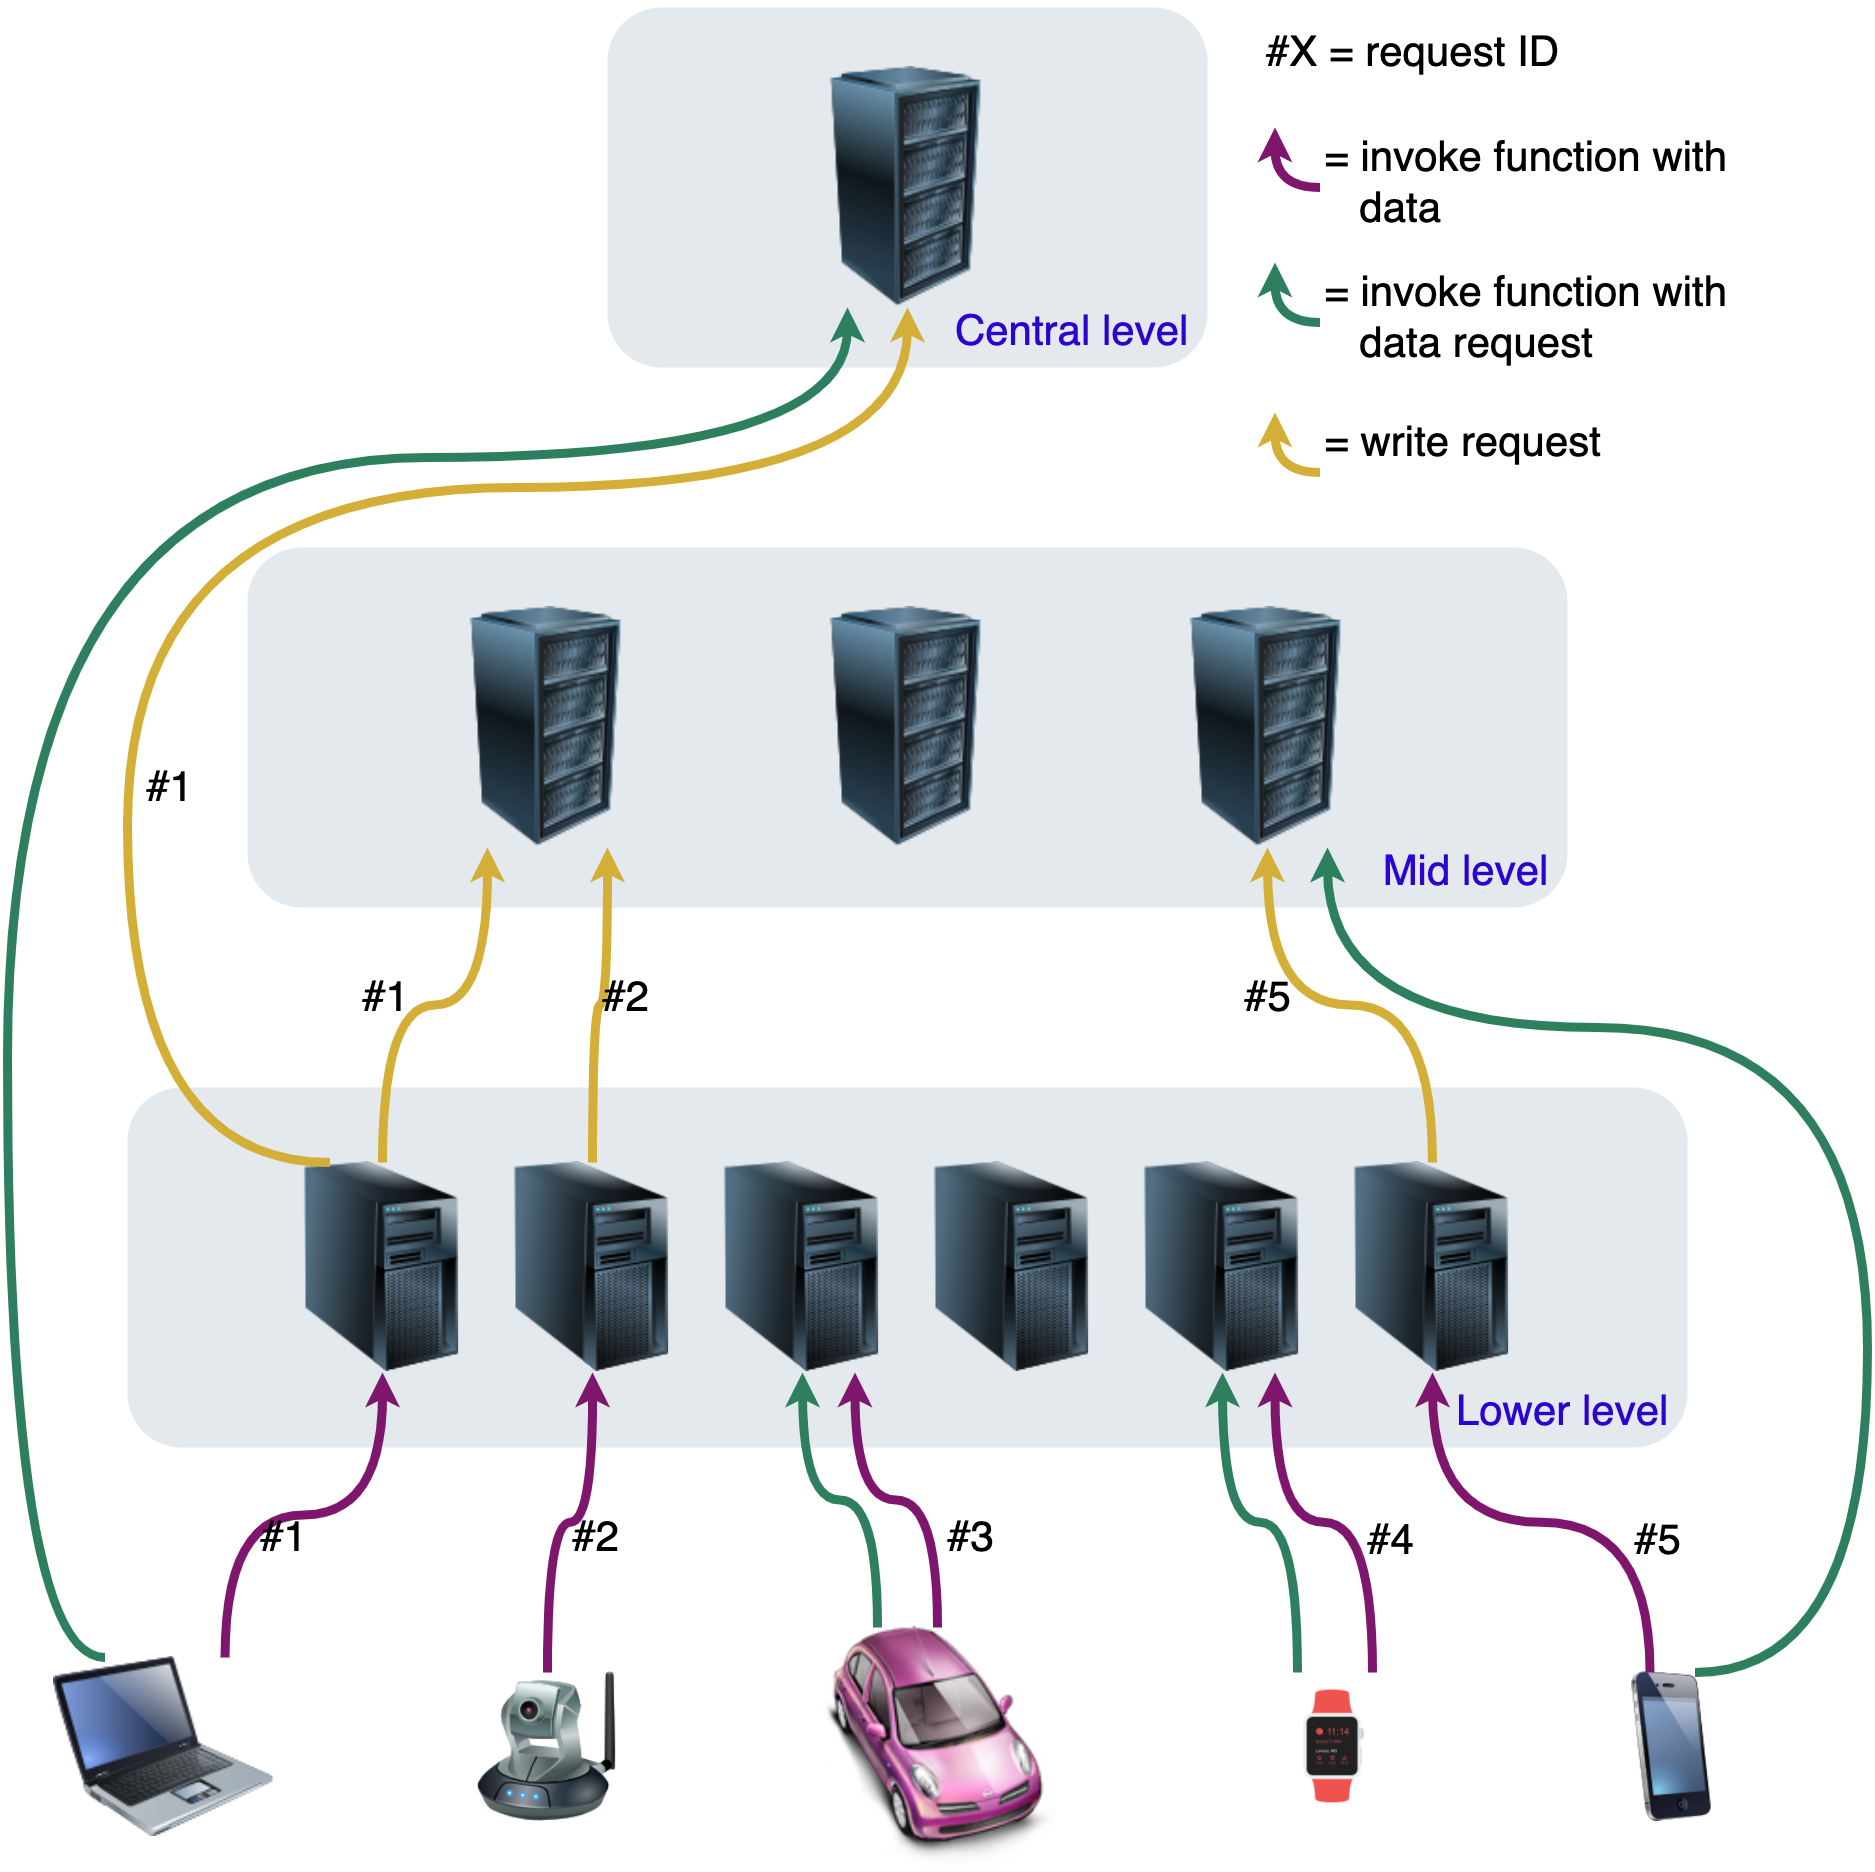
\includegraphics[width=0.99\linewidth]{Figures/Solution/high-level-architecture.png}
    \caption{High-level architecture of an example setup}
    \label{fig:high-level-architecture}
\end{figure}

In Figure \ref{fig:high-level-architecture} we show an example with three levels. Clients can \textbf{invoke functions} on the nearest location of a certain level, these functions can be used for both \textbf{sending data} or \textbf{requesting data}. When clients send data, the function written by the developer can process the data and then save the results in the provided stateful support. The results can be saved on different and multiple levels.


\subsection{Finding the Nearest Location}
Our solution assumes the presence of the ability to contact the \textbf{nearest server} automatically, without the intervention of the developer (the developer just needs to send the request to the function's URL).

This process has already been proved to be feasible and is in fact exploited by many web infrastructure companies to provide a Content Delivery Network or to provide serverless edge computing. The most common procedures to perform the process are the following:
\begin{itemize}
    \item \textbf{Anycast Routing}: this routing procedure uses the Border Gateway Protocol (BGP) to route clients using the natural network flow, indeed the information collected by the BGP protocol about network neighbors is used to efficiently route traffic based on hop count ensuring the shortest traveling distance between the client and its final destination \cite{anycast-cloudflare}.
    \item \textbf{Unicast Routing}: a process which can be incorporated into the standard Domain Name System (DNS) resolution process by using recursive DNS queries which redirect clients to the server closest to the DNS resolver (and usually the DNS resolver is physically near the client) \cite{unicast-vs-anycast}.
    \item \textbf{Manual Routing}: a procedure in which the client computes on its own which is the most appropriate server to contact, with this procedure GPS-equipped devices can use more precise information about the location.
\end{itemize}

In the implementation of our prototype we use a Manual Routing procedure where the clients would manually contact the nearest server, but in a real scenario a process like Unicast Routing or Anycast Routing could be preferred.


\subsection{Suitable Use Cases}
Our solution, for how has been thought, is suitable for use cases with the following characteristics:
\begin{itemize}
    \item \textbf{Stateful computation}: the use case needs a stateful support with \textbf{frequent writes} and reads.
    \item \textbf{Location awareness}: the use cases works on \textbf{geographic partitions} of the data;
    \item \textbf{Location is static}: data producers do not change location; OR \textbf{Location is dynamic but it’s not a problem to have a discontinuity in the data}: e.g., if there is an aggregation at the "city" level and a data producer exits the city, its data will have a discontinuity;
    \item \textbf{Session consistency is not needed}: the concept of session, where the user maintains consistency of the data even when the connected server changes, is not provided by our solution;
\end{itemize}

\chapter{The Prototype}
\label{ch:prototype}

In this chapter we will show the implementation of the prototype running the API that we presented in the previous chapter.

\section{The FaaS Platform}
We saw in Chapter \ref{ch:existing-solutions} the current frameworks to setup a FaaS platforms, we saw also a very valid implementation focused on edge use cases like the one of Cloudflare Workers, which can reach extremely fast cold-start latencies ($\approx$ 5ms), but unfortunately, being a proprietary solution, it cannot be applied in our framework.
So we resorted to an \textbf{open source} solution and we chose the solution provided by \textbf{OpenFaaS} since they provide two versions of their system, one version for high-performing machines with more overhead but that can scale greatly, and another more efficient version for edge devices with a smaller overhead but that cannot scale horizontally (there can only be one replica of the container running the function).


\subsection{Specifying Functions}
\label{subsec:specifying-functions}

We implemented two FaaS triggers in our prototype: an \textbf{HTTP trigger} (the function gets activated by a simple HTTP request) and the \textbf{cron trigger} (the function is automatically called periodically based on the current time). In practice the HTTP trigger is always present, and when the cron trigger is activated it periodically calls the relative HTTP endpoint of the function.

The following YAML code can be written to specify two functions, one with only the HTTP trigger, the other with the cron trigger:

\begin{lstlisting}[language=yaml,firstnumber=1]
functions:

  myHttpFunction:
    lang: node14
    handler: ./myHttpFunctionFolder
    image: dockerHubRef/myHttpFunction:latest
    limits:
      memory: 256Mi
      cpu: 1000m
    requests:
      memory: 4Mi
      cpu: 1m

  myCronFunction
    lang: node14
    handler: ./myCronFunctionFolder
    image: dockerHubRef/myCronFunction:latest
    limits:
      memory: 256Mi
      cpu: 1000m
    requests:
      memory: 4Mi
      cpu: 1m
    annotations:
      topic: cron-function
      schedule: */2 * * * *
\end{lstlisting}

We now analyze the example provided to better understand the architecture of our prototype. OpenFaas automatically scales and runs Docker images in response to HTTP requests; these Docker images execute the code provided by the developer.

The actual code is a \textbf{npm project} written in Node.js (in this case using Node version 14) placed in the folder specified in the \inlinecode{handler} section of the YAML. For example the function with name \inlinecode{myHttpFunction} has its code specified in the folder \inlinecode{./myHttpFunctionFolder}.
This code during deployment is compiled into a \textbf{Docker Image} and published to a \textbf{Docker Registry} (specified in \inlinecode{image} section of the YAML), so that machines that receive the deployment can pull the Docker Image from the Docker Registry and execute the function when requested.

OpenFaas adopted this architecture so that, when a function becomes idle for a lot of time and the machine is in need of resources, the cached Docker Image can be discarded since it can be easily re-obtained again from the Docker Registry.

In the YAML the developer can also specify the \textbf{CPU and RAM usage}. In the \inlinecode{limits} section of the YAML the developer can specify the maximum amount of RAM and CPU the instance can use, while in the \inlinecode{requests} section there can be specified the minimum amount of resources the machine must have free to run the instance.

Finally in the \inlinecode{annotations} section of the YAML the developer can optionally specify the cron trigger of the function with the standard Unix cron syntax \cite{cron-syntax}.


\section{Deployments}
We saw in the previous Chapter how our API can help the developer make precise deployments even on large scale networks thanks to the fields \inlinecode{inEvery}, \inlinecode{inAreas} and \inlinecode{exceptIn}. We implemented these fields in a \textbf{Command Line Interface} (CLI) that we built and which interacts with the APIs provided by OpenFaas to perform the deployment on the whole network.

To make any deployment we must first provide a way to specify the network with its hierarchy. The network can be specified by the web infrastructure company or by the developer (when using a proprietary network).


\subsection{Specifying the Hierarchy}
We provided a way to specify the hierarchy associated with the infrastructure by using the JavaScript Object Notation (JSON) format.
Below we provide an example of a hierarchy with 4 levels: continent, country, city, district.

\begin{lstlisting}[language=json,firstnumber=1]
{
  "areaTypesIdentifiers": ["continent", "country", "city", "district"],
  "hierarchy": {
    "europe": {
      "main-location": { },
      "italy": {
        "main-location": { },
        "milan": {
          "main-location": { },
          "milan001": { },
          "milan002": { }
        },
        "turin": {
          "main-location": { },
          "turin001": { },
          "turin002": { }
        }
      },
      "france": {
        "main-location": { },
        "paris": {
          "main-location": { },
          "paris001": { },
          "paris002": { }
        },
        "nice": {
          "main-location": { },
          "nice001": { },
          "nice002": { }
        }
      }
    }
  }
}
\end{lstlisting}

We used the \textbf{hierarchical structure} of JSON to represent the infrastructure hierarchy. In this example we have one "continent" location called "europe", containing two "country" locations called "italy" and "france", containing four "city" locations called "milan", "turin", "paris" and "nice", in turn containing eight "district" locations.

To simplify the visualization of the JSON we didn't show in this example the details of the machines associated to the areas; this information must be written in the places where two empty braces \inlinecode{\{ \}} are present. The fields that are inserted in the empty braces are the following:

\begin{itemize}
    \item \inlinecode{openfaas\_gateway}: the entrypoint for the OpenFaas API (e.g.,\\%Overfull
    "10.211.55.33:31112");
    \item \inlinecode{openfaas\_password}: the password for the OpenFaas entrypoint;
    \item \inlinecode{redis\_host}: the location that the code running in OpenFaas can use to access the Redis Database (e.g., "aaa.bbb.svc.cluster.local");
    \item \inlinecode{redis\_port}: the port that the Redis Database is using (e.g., "6379");
    \item \inlinecode{redis\_password}: the password for accessing the Redis Database;
\end{itemize}


\subsection{The Command Line Interface}
The CLI can then be used by the developer to perform the actual \textbf{deployment}.
By issuing the command \inlinecode{deployer deploy --help}, the CLI shows the usage of the "deploy" command:

\begin{lstlisting}[language=bash]
Usage: deployer deploy [options] <functionName> <infrastructure>

Deploys the function to the infrastructure specified.

Options:
  --inEvery <areaTypeIdentifier>  In which area type to deploy the function. If not specified the function is deployed to the lowest level.
  --inAreas <areas...>            The name of the areas in which to deploy the function. If not specified the function is deployed everywhere.
  --exceptIn <areas...>           The name of the areas in which to NOT deploy the function.
  -f, --yaml <path>               Path to the YAML file describing the function. (default: "stack.yml")
\end{lstlisting}

For the "deploy" command two fields are required, the \inlinecode{functionName} field specifying which function to be deployed and the \inlinecode{infrastructure} field specifying the path to the infrastructure JSON.
Then we have the \inlinecode{inEvery}, \inlinecode{inAreas} and \inlinecode{exceptIn} fields that are used to specify where to make the deployments (if some of these fields are not specified a default value is assumed).
And at last the \inlinecode{yaml} field is used to specify the path to the YAML file describing the function as seen in Subsection \ref{subsec:specifying-functions}.

To better understand how the CLI works we now present an example:

\begin{lstlisting}[language=bash]
deployer deploy myHttpFunction infrastructure.json --inEvery district --inAreas italy paris --exceptIn milan paris001 --yaml stack.yml
\end{lstlisting}

In this example the function called \inlinecode{myHttpFunction}, specified in the YAML file \inlinecode{stack.yml}, is deployed to the infrastructure. The function is deployed at the \inlinecode{district} level in all the districts contained in the areas of \inlinecode{italy} and \inlinecode{paris}, but excluding the districts contained in the area of \inlinecode{milan} and excluding the district \inlinecode{paris001}.

The CLI first analyzes the infrastructure and the deployment locations specified with the fields \inlinecode{inEvery}, \inlinecode{inAreas} and \inlinecode{exceptIn}. After listing all the locations where the deploy is needed the CLI builds the code of the function into a Docker Image, then it publishes the Docker Image to the Docker Registry and finally performs the actual deployments by calling the OpenFaas API of the machines running in the locations collected.


\section{Stateful Support}
To provide support for stateful computations we created an API that interacts with a \textbf{Redis instance} running on the machine.
In our prototype we run the Redis container (a Docker Image) as a Persistent Volume on the container-orchestration system that runs OpenFaas.


\subsection{Reads and Writes}

For allowing the developer to make writes and reads on the Redis instance we wrote a JavaScript API that can be added as a \textbf{dependency} in the npm project of a function.
In this early prototype we provided the following APIs:

\begin{itemize}
    \item \textit{get}: gets the value associated to a key;
    \item \textit{getList}: gets the list of values associated to the key;
    \item \textit{set}: sets the key to hold the provided value;
    \item \textit{addToList}: adds a value to the list specified by the key (if the list does not exists it is automatically created).
\end{itemize}
The two "read" APIs allow only to read the values that the current location contains, so if the developer wants to access "continent" level data, the developer will need to deploy a function at the "continent" level and perform a get operation in the function. 
While the two write APIs allow saving the data on one or multiple levels. Since the processing should be done on a lower level so that it is performed as close as possible to the user, these APIs only allow forwarding data on upper levels. In every write action there must also be specified a Time-To-Live that will be applied to that value, this forces developers to not accumulate data in the stateful support. Accumulating data should be avoided due to the more bounded resources present at the edge of the network.


\subsubsection{Get}
The provided \textit{get} API uses the parameters reported below:

\begin{itemize}
    \item \inlinecode{key}: the key to be used for getting the value associated to it.
\end{itemize}

\begin{example}
Get the value associated to the key "my\_key1".
\begin{lstlisting}[language=javascript]
const edgeDb = require('edge-db');
const value = await edgeDb.get("my_key1");
\end{lstlisting}
\end{example}


\subsubsection{GetList}
The provided \textit{getList} API uses the parameters reported below:

\begin{itemize}
    \item \inlinecode{key}: the key to be used for getting the list associated to it.
\end{itemize}

\begin{example}
Get the list associated to the key "my\_list1".
\begin{lstlisting}[language=javascript]
const edgeDb = require('edge-db');
const list = await edgeDb.getList("my_list1");
\end{lstlisting}
\end{example}


\subsubsection{Set}
The provided \textit{set} API uses the parameters reported below:

\begin{itemize}
    \item \inlinecode{referringAreaType}: the identifier of the level in the hierarchy where we want the aggregation to happen (e.g., "district", "city", "country").
    \item \inlinecode{saveAlsoInIntermediateLevels}: a boolean that if set to true will save the value to all levels starting from the current level where the function is deployed, up until the level specified in \inlinecode{referringAreaType}. If false the value will be only saved at the level specified in \inlinecode{referringAreaType}.
    \item \inlinecode{ttl}: the Time-To-Live of the value.
    \item \inlinecode{key}: the key where to save the value.
    \item \inlinecode{data}: the value to be saved.
\end{itemize}

The \textit{set} API also offers two optional parameters for some more advanced configurations:
\begin{itemize}
    \item \inlinecode{onlySetIfKeyDoesNotAlreadyExist}: set to true if the write should be performed only if the key does not already exist.
    \item \inlinecode{onlySetIfKeyAlreadyExist}: set to true if the write should be performed only if the key already exists.
\end{itemize}

\begin{example}
Suppose the function is to be deployed in the "city" level. Here we set the value of the key "my\_key1" equal to "myValue1".
\begin{lstlisting}[language=javascript]
const edgeDb = require('edge-db');
const dataDomain = { referringAreaType: "continent", saveAlsoInIntermediateLevels: false, ttl: 60*60*1000 };
const isSuccess = await edgeDb
    .withDataDomain(dataDomain)
    .set("my_key1", "myValue1");
\end{lstlisting}
The \inlinecode{referringAreaType} is set to "continent" and the write happened with the \inlinecode{saveAlsoInIntermediateLevels} boolean set to false, so the write will be only performed on the corresponding "continent" location.
\end{example}

\begin{example}
Suppose the function is to be deployed in the "city" level and that the levels in the hierarchy are the following in an increasing order of size: "district", "city", "country", "continent". Here we set the value of the key "my\_key1" equal to "myValue2".
\begin{lstlisting}[language=javascript]
const edgeDb = require('edge-db');
const dataDomain = { referringAreaType: "continent", saveAlsoInIntermediateLevels: true, ttl: 60*60*1000 };
const isSuccess = await edgeDb
    .withDataDomain(dataDomain)
    .set("my_key1", "myValue2");
\end{lstlisting}
The \inlinecode{referringAreaType} is set to "continent" and the write happened with the \inlinecode{saveAlsoInIntermediateLevels} boolean set to true, so the write will be performed on the corresponding "city", "country" and "continent" locations.
\end{example}


\subsubsection{AddToList}
The provided \textit{addToList} API uses the parameters reported below:

\begin{itemize}
    \item \inlinecode{referringAreaType}: the identifier of the level in the hierarchy where we want the aggregation to happen (e.g., "district", "city", "country").
    \item \inlinecode{saveAlsoInIntermediateLevels}: a boolean that if set to true will save the value to all levels starting from the current level where the function is deployed, up until the level specified in \inlinecode{referringAreaType}. If false the value will be only saved at the level specified in \inlinecode{referringAreaType}.
    \item \inlinecode{ttl}: the Time-To-Live of the value.
    \item \inlinecode{key}: the key associated to the list.
    \item \inlinecode{data}: the value to be saved in the list.
\end{itemize}

\begin{example}
Suppose the function is to be deployed in the "city" level. Here we add the value "myValue1" to the list specified by the key "my\_list1".
\begin{lstlisting}[language=javascript]
const edgeDb = require('edge-db');
const dataDomain = { referringAreaType: "continent", saveAlsoInIntermediateLevels: false, ttl: 60*60*1000 };
const isSuccess = await edgeDb
    .withDataDomain(dataDomain)
    .addToList("my_list1", "myValue1");
\end{lstlisting}
The \inlinecode{referringAreaType} is set to "continent" and the write happened with the \inlinecode{saveAlsoInIntermediateLevels} boolean set to false, so the value "myValue1" will be only added to the list "my\_list1" present in the corresponding "continent" location.
\end{example}

\begin{example}
Suppose the function is to be deployed in the "city" level and that the levels in the hierarchy are the following in an increasing order of size: "district", "city", "country", "continent". Here we add the value "myValue2" to the list specified by the key "my\_list1".
\begin{lstlisting}[language=javascript]
const edgeDb = require('edge-db');
const dataDomain = { referringAreaType: "continent", saveAlsoInIntermediateLevels: true, ttl: 60*60*1000 };
const isSuccess = await edgeDb
    .withDataDomain(dataDomain)
    .addToList("my_list1", "myValue2");
\end{lstlisting}
The \inlinecode{referringAreaType} is set to "continent" and the write happened with the \inlinecode{saveAlsoInIntermediateLevels} boolean set to true, so the value "myValue2" will be added to the list "my\_list1" present in the corresponding "city", "country" and "continent" locations.
\end{example}


\subsection{Internal Communication}
In some of the write calls, locations need to \textbf{communicate internally} to exchange the data. For example in a scenario where a simple "set" is performed at the "city" level with \inlinecode{referringAreaType} equal to "continent", the \inlinecode{edge-db} needs to forward the data to the corresponding "continent" location. In our solution this exchange only happens starting from a location of a lower level, going into a location of an upper level. There is no internal communication happening up-to-down or mid-level.

To implement the communication we chose to use the same OpenFaas system used for running functions written by the developer: we implemented an \textbf{HTTP-triggered function} that receives the data and can save it in the database of the location.
Having a function makes the architecture more modular, and it will be easier to add filters or a more advanced authentication to the communication.


\section{Applying the Prototype to Use Cases}
\label{sec:prototype_applying_to_use_cases}
In this section we show a few examples where we apply our solutions to solve the same use cases that we presented in Section \ref{sec:solution_use_cases}.

\subsubsection{IoT Data Compression}
As we showed, in this use case we are trying to compress the data of IoT sensors by sending only significant value changes.

This has been done by developing a stateful function that checks whether the new value is equal to the previous value:

Function code (placed in the folder "iot-data-reduction"):
\begin{lstlisting}[language=javascript]
const edgeDb = require("edge-db");
const ioTDataDomain = { referringAreaType: "location", saveAlsoInIntermediateLevels: false, ttl: 5*24*60*60*1000 }; // 5 days TTL.

module.exports = async (event, context) => {
  const iotData = event.body.iot_data;
  const sensorName = event.body.sensor_name;
  const previousIotData = await edgeDb.get("latest_data_of_" + sensorName);

  if(iotData !== previousIotData) {
    await edgeDb
      .withDataDomain(ioTDataDomain)
      .set("latest_data_of_" + sensorName, iotData);
        
    // Send value to the cloud.

    return context
        .status(200)
        .succeed('Value updated.');
  } else {
    return context
        .status(200)
        .succeed('Value not changed.');
  }
}
\end{lstlisting}

Function specification:
\begin{lstlisting}[language=yaml,firstnumber=1]
functions:

  iot-data-reduction:
    lang: node14
    handler: ./iot-data-reduction
    image: dockerHubRef/iot-data-reduction:latest
    limits:
      memory: 256Mi
      cpu: 1000m
    requests:
      memory: 4Mi
      cpu: 0m
\end{lstlisting}

Deployment command:
\begin{lstlisting}[language=bash]
deployer deploy iot-data-reduction infrastructure.json --inEvery building --inAreas factory1 factory2
\end{lstlisting}

Essentially we developed a stateful function that compares the saved value of a sensor with the current value, and if different this value gets updated and forwarded to the cloud.


\subsubsection{Road Traffic Monitoring}
As we showed, in this use case we analyze video footage data to get an insight on the road traffic and then use such insight in an algorithm to find the fastest path between two points.

It has been implemented by using two functions: an HTTP trigger that receives data from the cameras, converts the footage in a value of traffic and finally saves this value; and another HTTP trigger that is called by the user when interested in obtaining the fastest path between two points.

Code of the first function (placed in the folder "video-footage-receiver"):
\begin{lstlisting}[language=javascript]
const edgeDb = require("edge-db");
const trafficStatusDataDomain = { referringAreaType: "central", saveAlsoInIntermediateLevels: true, ttl: 30*60*1000 }; // 30 minutes TTL.

module.exports = async (event, context) => {
  const videoFootageData = event.body.footage_data;
  const cameraId = event.body.camera_id;
  const trafficStatus = await analyzeCrowdStatus(videoFootageData);
  const response = await edgeDb
      .withDataDomain(trafficStatusDataDomain)
      .set("traffic_" + cameraId, trafficStatus);
  return context
      .status(200)
      .succeed(response);
}
\end{lstlisting}

Code of the second function (placed in the folder "get-fastest-path"):
\begin{lstlisting}[language=javascript]
const edgeDb = require("edge-db");

module.exports = async (event, context) => {
  const startingPoint = event.body.starting_point;
  const destinationPoint = event.body.destination_point;

  const cameraIds = await getCameraIdsForPossiblePaths(startingPoint, destinationPoint);
  const trafficStatuses = [];
  for(const cameraId of cameraIds) {
    const trafficStatus = await edgeDb.get("traffic_" + cameraId);
    if(trafficStatus === null || trafficStatus === undefined)
      trafficStatuses.push(1.0);
    else
      trafficStatuses.push(trafficStatus);
  }

  const bestPath = await computeBestPath(cameraIds, trafficStatuses);

  return context
      .status(200)
      .succeed(bestPath);
}
\end{lstlisting}

Functions specification:
\begin{lstlisting}[language=yaml,firstnumber=1]
functions:

  video-footage-receiver:
    lang: node14
    handler: ./video-footage-receiver
    image: dockerHubRef/video-footage-receiver
    limits:
      memory: 256Mi
      cpu: 500m
    requests:
      memory: 4Mi
      cpu: 0m
      
  get-fastest-path:
    lang: node14
    handler: ./get-fastest-path
    image: dockerHubRef/get-fastest-path
    limits:
      memory: 256Mi
      cpu: 1000m
    requests:
      memory: 4Mi
      cpu: 0m
\end{lstlisting}

Deployment commands:
\begin{lstlisting}[language=bash]
deployer deploy video-footage-receiver infrastructure.json --inEvery district --inAreas us

deployer deploy get-fastest-path infrastructure.json --inEvery city --inAreas us

deployer deploy get-fastest-path infrastructure.json --inEvery country --inAreas us
\end{lstlisting}


\subsubsection{Trending Topics}
As we showed, in this use case we want to find the trending topics in a certain region in an application (like trending users in a social network, or trending searches).

It has been implemented using two functions: an HTTP trigger that receives the topics from the users and aggregates the data; and a cron trigger that gets called periodically to find the trending topics from the list of topics present in the region.

Code of the HTTP-triggered function (placed in the folder "search-analytics-data-receiver"):
\begin{lstlisting}[language=javascript]
const edgeDb = require("edge-db");
const trendingSearchesDataDomain = { referringAreaType: "country", saveAlsoInIntermediateLevels: true, ttl: 4*60*60*1000  }; // 4 hours TTL.

module.exports = async (event, context) => {
  const searchData = event.body.search_data.toLowerCase();
  const response = await edgeDb
      .withDataDomain(trendingSearchesDataDomain)
      .addToList("latest_searches_list", searchData);
  return context
      .status(200)
      .succeed(response);
}
\end{lstlisting}

Code of the cron-triggered function (placed in the folder "search-analytics-performer"):
\begin{lstlisting}[language=javascript]
const edgeDb = require("edge-db");

module.exports = async (event, context) => {
  const latestSearchesList = await edgeDb.getList("latest_searches_list");

  const trendingSearches = await getTrendingSearches(latestSearchesList);

  return context
      .status(200)
      .succeed(trendingSearches);
}

async function getTrendingSearches(latestSearchesList) {
  // Compute trending searches from searches list.
}
\end{lstlisting}

Functions specification:
\begin{lstlisting}[language=yaml,firstnumber=1]
functions:

  search-analytics-data-receiver:
    lang: node14
    handler: ./search-analytics-data-receiver
    image: dockerHubRef/search-analytics-data-receiver
    limits:
      memory: 256Mi
      cpu: 1000m
    requests:
      memory: 4Mi
      cpu: 0m

  search-analytics-performer:
    lang: node14
    handler: ./search-analytics-performer
    image: dockerHubRef/search-analytics-performer
    limits:
      memory: 256Mi
      cpu: 1000m
    requests:
      memory: 4Mi
      cpu: 0m
    annotations:
      topic: cron-function
      schedule: "0,30 * * * *"
\end{lstlisting}

Deployment commands:
\begin{lstlisting}[language=bash]
deployer deploy search-analytics-data-receiver infrastructure.json --inEvery city

deployer deploy search-analytics-performer infrastructure.json --inEvery territory
\end{lstlisting}

\section{Experimental evaluation}
\label{sec:evaluation}

We performed two types of evaluation: a first assessment done on the \textbf{working prototype} running on multiple Virtual Machines (VMs) and an evaluation using simulations run on a \textbf{discrete-event simulator}.
In the first case, since it's not possible to emulate a network similar to a real edge network due to the amount of resources needed, we focus on the \textbf{effectiveness}, \textbf{efficiency} and \textbf{usability} of the framework.
While with the discrete-event simulation at hand we can focus on the \textbf{latency} and the \textbf{bandwidth} consumed.


\subsection{Performance}
We found that, after paying the \textbf{cold-start} price where the initialization of the container running the function would create a noticeable latency, functions were executed in milliseconds even when using the (local) stateful support. This speed of the stateful support has been possible thanks to the usage of an in-memory database like Redis.

We also tested the \textbf{scalability} of our solution when using the \textit{faas} flavour of OpenFaas: we made 10'000 sequential calls to a node running a simple function and we noticed that new containers were immediately created to fulfill the stream of requests. After the 10'000 calls ended and no new calls were made, OpenFaas automatically scaled down and brought the number of idle containers to one.


\subsection{Usability}
We tested our solution with the implementation of some use cases.
Our solution allows developers to forget about the location, which instead is handled internally, and forget about handling the complex management of hundreds of geo-distributed nodes.
This avoids the creation of custom solutions that overfit on the available infrastructure, creating a code that becomes task-specific and difficult to extend and maintain.
In fact, developers would need to set up the infrastructure all by themselves, a process which can create errors or malfunctions, while the serverless FaaS architecture in our solution allows to forget about the handling of the infrastructure.

\subsection{Simulation Summary}
Thanks to the various experiments performed on the simulation we showed that by using our framework we get immense benefits in terms of \textbf{reduced traffic} in the network (Figure \ref{fig:write-by-traffic1}) while allowing \textbf{faster reads} when the data aggregation needed is not central.

\begin{figure}
    \centering
    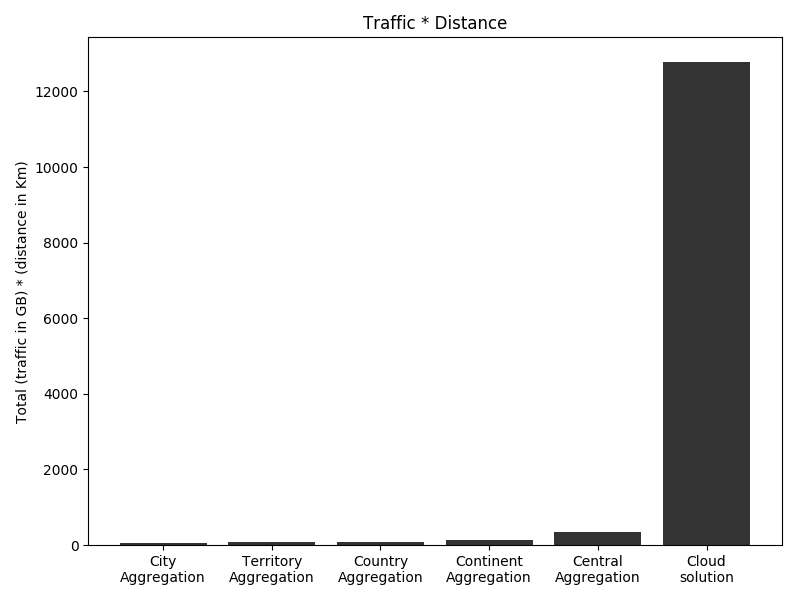
\includegraphics[width=0.99\linewidth]{Figures/Evaluation/write-by-traffic1-simplified.png}
    \caption{Traffic per distance generated in the network.}
    \label{fig:write-by-traffic1}
\end{figure}

\iffalse
\begin{figure}
    \centering
    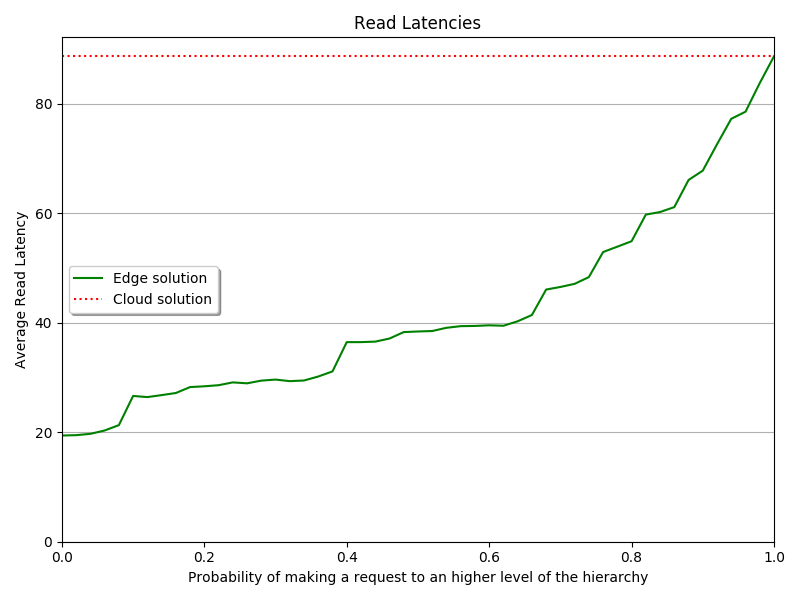
\includegraphics[width=0.99\linewidth]{Figures/Evaluation/read-all-latency.png}
    \caption{Average read latency as a function of the probability of making the read request to an higher level}
    \label{fig:read-all-latency}
\end{figure}
\fi

In a case where a central aggregation is still needed we showed that the write requests suffer an increase in latency, but the increase is not substantial ($\approx$139ms on the simulation of our approach, versus the $\approx$109ms on the simulation of the cloud solution).

During the simulations we also noticed how our edge solution can be affected by an increase in the average write latency due to random spikes in the requests. This is caused by the small number of cores and resources in the lowest level of the hierarchy that can't keep up with the spike of requests. Fortunately this increase is not drastic.

\chapter{Conclusions and Future Developments}
\label{ch:conclusions}


\section{Conclusions}
The large diffusion of smart devices and IoT sensors has resulted in an \textbf{unprecedented growth} in the amount of collected data. Core-centric approaches have shown to be inefficient as they need to transfer data back and forth between the core and the devices, generating notable latencies. Therefore new approaches, which exploit the \textbf{tremendous power of the edge} of the network, are replacing the core-centric approaches.

In this thesis we have studied the problem of performing \textbf{stateful computations in a geo-distributed and heterogeneous scenario}, that is the edge of the network.

After analyzing the state of the art in the literature, we defined key research questions that guided our research.
We started by \textbf{collecting and organizing the use cases} predominantly affected by bandwidth and latency constraints. With the use cases at hand we \textbf{studied the current frameworks} provided by the industry and we noticed that some of the use cases were left out and couldn't be fulfilled by the available frameworks. This situation forces developers to create ad hoc solutions on the infrastructure, a process which is error-prone and task-specific.

Therefore we tried to solve the gap of fulfillment present in the use cases, by proposing a \textbf{new solution} which supports the characteristics of the use cases left out. We designed and then implemented a \textbf{prototype} for this solution which brings stateful computations and location awareness in contexts where a change of location of the clients does not occur or is not important (the solution in fact does not provide session consistency).

We then \textbf{evaluated} the performance and usability of our prototype in a simple scenario. Instead to evaluate the solution in a complex but more realistic scenario we resorted to a \textbf{discrete-event simulation}.
We found that, by using our framework with the right use cases, we get immense benefits in terms of \textbf{reduced traffic} in the network and in terms of \textbf{lower latencies}, especially in cases where the data aggregation needed is not central. However we also noticed how our solution can be affected by a latency increase due to random spikes in the requests and due to the small number of cores and resources at the edge of the network. Nevertheless the results of the evaluation confirmed the \textbf{power and effectiveness of the proposed solution}.


\section{Future Developments}
In this thesis, we have addressed several key issues related to stateful serverless computing on the edge by designing and implementing a new solution. However, with our solution, not every use case can be fulfilled, in fact the absence of \textbf{session consistency} makes the usage impractical in a dynamic context where the location of the client changes.
Therefore a possible improvement and a possible research direction could be session consistency in the context of stateful serverless computing on the edge.

Another problem with our solution is the possibility for edge locations to be overwhelmed due to random spikes in requests targeting a specific location: our solution does not support the \textbf{offload of the computation} to free up some resources from an overloaded node. On the contrary, for how we thought our solution, in some use cases it's important to be static and to always reach the same node. 

In the context of serverless computing a common problem is the phenomenon of \textbf{cold-start}, which impacts processing latency. As we saw, there exist solutions that firmly mitigated the problem reaching milliseconds cold-start latencies (Cloudflare Workers), but unfortunately these solutions are currently proprietary.

\section{Future Developments}
\label{sec:future_developments}

In this thesis, we have addressed several key issues related to stateful serverless computing on the edge by designing and implementing a new solution. However, with our solution, not every use case can be fulfilled, in fact the absence of \textbf{session consistency} makes the usage impractical in a dynamic context where the location of the client changes.
Therefore a possible improvement and a possible research direction could be session consistency in the context of stateful serverless computing on the edge.

Another problem with our solution is the possibility for edge locations to be overwhelmed due to random spikes in requests targeting a specific location: our solution does not support the \textbf{offload of the computation} to free up some resources from an overloaded node. On the contrary, for how we thought our solution, in some use cases it's important to be static and to always reach the same node. 

In the context of serverless computing a common problem is the phenomenon of \textbf{cold-start}, which impacts processing latency. There exist solutions that firmly mitigated the problem reaching milliseconds cold-start latencies (like the solution provided by Cloudflare Workers), but unfortunately these solutions are currently proprietary.


\chapter{Acknowledgements}
In this chapter, you can acknowledge the people that were somehow helpful in the realization of the thesis. It is better to keep this chapter formal, you can add the friendly thanks at the end (chapter Thanks).

%---------------------------------------------------------------------------
%  BIBLIOGRAPHY
%---------------------------------------------------------------------------
% Remember to insert here only the essential bibliography of your work
\bibliography{bibliography.bib} % automatically inserted and ordered with this command 

\end{document}